% Created by tikzDevice version 0.12.3.1 on 2021-09-17 14:36:13
% !TEX encoding = UTF-8 Unicode
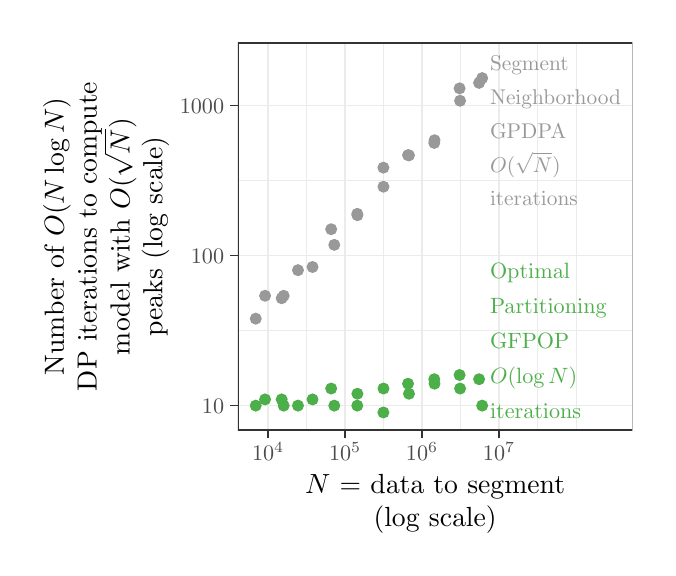
\begin{tikzpicture}[x=1pt,y=1pt]
\definecolor{fillColor}{RGB}{255,255,255}
\path[use as bounding box,fill=fillColor,fill opacity=0.00] (0,0) rectangle (224.04,187.90);
\begin{scope}
\path[clip] (  0.00,  0.00) rectangle (224.04,187.90);
\definecolor{drawColor}{RGB}{255,255,255}
\definecolor{fillColor}{RGB}{255,255,255}

\path[draw=drawColor,line width= 0.6pt,line join=round,line cap=round,fill=fillColor] (  0.00, -0.00) rectangle (224.04,187.90);
\end{scope}
\begin{scope}
\path[clip] ( 75.93, 42.49) rectangle (218.54,182.40);
\definecolor{fillColor}{RGB}{255,255,255}

\path[fill=fillColor] ( 75.93, 42.49) rectangle (218.54,182.40);
\definecolor{drawColor}{gray}{0.92}

\path[draw=drawColor,line width= 0.3pt,line join=round] ( 75.93, 78.43) --
	(218.54, 78.43);

\path[draw=drawColor,line width= 0.3pt,line join=round] ( 75.93,132.63) --
	(218.54,132.63);

\path[draw=drawColor,line width= 0.3pt,line join=round] (100.77, 42.49) --
	(100.77,182.40);

\path[draw=drawColor,line width= 0.3pt,line join=round] (128.59, 42.49) --
	(128.59,182.40);

\path[draw=drawColor,line width= 0.3pt,line join=round] (156.41, 42.49) --
	(156.41,182.40);

\path[draw=drawColor,line width= 0.3pt,line join=round] (184.23, 42.49) --
	(184.23,182.40);

\path[draw=drawColor,line width= 0.3pt,line join=round] (198.14, 42.49) --
	(198.14,182.40);

\path[draw=drawColor,line width= 0.6pt,line join=round] ( 75.93, 51.33) --
	(218.54, 51.33);

\path[draw=drawColor,line width= 0.6pt,line join=round] ( 75.93,105.53) --
	(218.54,105.53);

\path[draw=drawColor,line width= 0.6pt,line join=round] ( 75.93,159.73) --
	(218.54,159.73);

\path[draw=drawColor,line width= 0.6pt,line join=round] ( 86.86, 42.49) --
	( 86.86,182.40);

\path[draw=drawColor,line width= 0.6pt,line join=round] (114.68, 42.49) --
	(114.68,182.40);

\path[draw=drawColor,line width= 0.6pt,line join=round] (142.50, 42.49) --
	(142.50,182.40);

\path[draw=drawColor,line width= 0.6pt,line join=round] (170.32, 42.49) --
	(170.32,182.40);
\definecolor{drawColor}{gray}{0.60}
\definecolor{fillColor}{gray}{0.60}

\path[draw=drawColor,line width= 0.4pt,line join=round,line cap=round,fill=fillColor] ( 82.41, 82.75) circle (  1.96);

\path[draw=drawColor,line width= 0.4pt,line join=round,line cap=round,fill=fillColor] ( 85.78, 91.02) circle (  1.96);

\path[draw=drawColor,line width= 0.4pt,line join=round,line cap=round,fill=fillColor] ( 91.78, 90.13) circle (  1.96);

\path[draw=drawColor,line width= 0.4pt,line join=round,line cap=round,fill=fillColor] ( 92.51, 91.02) circle (  1.96);

\path[draw=drawColor,line width= 0.4pt,line join=round,line cap=round,fill=fillColor] ( 97.67,100.27) circle (  1.96);

\path[draw=drawColor,line width= 0.4pt,line join=round,line cap=round,fill=fillColor] (102.94,101.42) circle (  1.96);

\path[draw=drawColor,line width= 0.4pt,line join=round,line cap=round,fill=fillColor] (109.67,115.07) circle (  1.96);

\path[draw=drawColor,line width= 0.4pt,line join=round,line cap=round,fill=fillColor] (110.79,109.42) circle (  1.96);

\path[draw=drawColor,line width= 0.4pt,line join=round,line cap=round,fill=fillColor] (119.10,120.63) circle (  1.96);

\path[draw=drawColor,line width= 0.4pt,line join=round,line cap=round,fill=fillColor] (119.15,120.13) circle (  1.96);

\path[draw=drawColor,line width= 0.4pt,line join=round,line cap=round,fill=fillColor] (128.54,137.32) circle (  1.96);

\path[draw=drawColor,line width= 0.4pt,line join=round,line cap=round,fill=fillColor] (128.57,130.43) circle (  1.96);

\path[draw=drawColor,line width= 0.4pt,line join=round,line cap=round,fill=fillColor] (137.44,141.85) circle (  1.96);

\path[draw=drawColor,line width= 0.4pt,line join=round,line cap=round,fill=fillColor] (137.78,141.75) circle (  1.96);

\path[draw=drawColor,line width= 0.4pt,line join=round,line cap=round,fill=fillColor] (146.92,146.25) circle (  1.96);

\path[draw=drawColor,line width= 0.4pt,line join=round,line cap=round,fill=fillColor] (147.02,147.23) circle (  1.96);

\path[draw=drawColor,line width= 0.4pt,line join=round,line cap=round,fill=fillColor] (156.07,165.97) circle (  1.96);

\path[draw=drawColor,line width= 0.4pt,line join=round,line cap=round,fill=fillColor] (156.25,161.49) circle (  1.96);

\path[draw=drawColor,line width= 0.4pt,line join=round,line cap=round,fill=fillColor] (163.12,167.95) circle (  1.96);

\path[draw=drawColor,line width= 0.4pt,line join=round,line cap=round,fill=fillColor] (164.23,169.68) circle (  1.96);
\definecolor{drawColor}{RGB}{77,175,74}
\definecolor{fillColor}{RGB}{77,175,74}

\path[draw=drawColor,line width= 0.4pt,line join=round,line cap=round,fill=fillColor] ( 82.41, 51.33) circle (  1.96);

\path[draw=drawColor,line width= 0.4pt,line join=round,line cap=round,fill=fillColor] ( 85.78, 53.57) circle (  1.96);

\path[draw=drawColor,line width= 0.4pt,line join=round,line cap=round,fill=fillColor] ( 91.78, 53.57) circle (  1.96);

\path[draw=drawColor,line width= 0.4pt,line join=round,line cap=round,fill=fillColor] ( 92.51, 51.33) circle (  1.96);

\path[draw=drawColor,line width= 0.4pt,line join=round,line cap=round,fill=fillColor] ( 97.67, 51.33) circle (  1.96);

\path[draw=drawColor,line width= 0.4pt,line join=round,line cap=round,fill=fillColor] (102.94, 53.57) circle (  1.96);

\path[draw=drawColor,line width= 0.4pt,line join=round,line cap=round,fill=fillColor] (109.67, 57.50) circle (  1.96);

\path[draw=drawColor,line width= 0.4pt,line join=round,line cap=round,fill=fillColor] (110.79, 51.33) circle (  1.96);

\path[draw=drawColor,line width= 0.4pt,line join=round,line cap=round,fill=fillColor] (119.10, 51.33) circle (  1.96);

\path[draw=drawColor,line width= 0.4pt,line join=round,line cap=round,fill=fillColor] (119.15, 55.62) circle (  1.96);

\path[draw=drawColor,line width= 0.4pt,line join=round,line cap=round,fill=fillColor] (128.54, 48.85) circle (  1.96);

\path[draw=drawColor,line width= 0.4pt,line join=round,line cap=round,fill=fillColor] (128.57, 57.50) circle (  1.96);

\path[draw=drawColor,line width= 0.4pt,line join=round,line cap=round,fill=fillColor] (137.44, 59.25) circle (  1.96);

\path[draw=drawColor,line width= 0.4pt,line join=round,line cap=round,fill=fillColor] (137.78, 55.62) circle (  1.96);

\path[draw=drawColor,line width= 0.4pt,line join=round,line cap=round,fill=fillColor] (146.92, 60.87) circle (  1.96);

\path[draw=drawColor,line width= 0.4pt,line join=round,line cap=round,fill=fillColor] (147.02, 59.25) circle (  1.96);

\path[draw=drawColor,line width= 0.4pt,line join=round,line cap=round,fill=fillColor] (156.07, 62.39) circle (  1.96);

\path[draw=drawColor,line width= 0.4pt,line join=round,line cap=round,fill=fillColor] (156.25, 57.50) circle (  1.96);

\path[draw=drawColor,line width= 0.4pt,line join=round,line cap=round,fill=fillColor] (163.12, 60.87) circle (  1.96);

\path[draw=drawColor,line width= 0.4pt,line join=round,line cap=round,fill=fillColor] (164.23, 51.33) circle (  1.96);
\end{scope}
\begin{scope}
\path[clip] ( 75.93, 42.49) rectangle (218.54,182.40);
\definecolor{drawColor}{RGB}{77,175,74}

\node[text=drawColor,anchor=base west,inner sep=0pt, outer sep=0pt, scale=  0.80] at (167.07, 97.44) {Optimal};

\node[text=drawColor,anchor=base west,inner sep=0pt, outer sep=0pt, scale=  0.80] at (167.07, 84.77) {Partitioning};

\node[text=drawColor,anchor=base west,inner sep=0pt, outer sep=0pt, scale=  0.80] at (167.07, 72.10) {GFPOP};

\node[text=drawColor,anchor=base west,inner sep=0pt, outer sep=0pt, scale=  0.80] at (167.07, 59.43) {$O(\log N)$};

\node[text=drawColor,anchor=base west,inner sep=0pt, outer sep=0pt, scale=  0.80] at (167.07, 46.75) {iterations};
\definecolor{drawColor}{gray}{0.60}

\node[text=drawColor,anchor=base west,inner sep=0pt, outer sep=0pt, scale=  0.77] at (167.07,172.33) {Segment};

\node[text=drawColor,anchor=base west,inner sep=0pt, outer sep=0pt, scale=  0.77] at (167.07,160.13) {Neighborhood};

\node[text=drawColor,anchor=base west,inner sep=0pt, outer sep=0pt, scale=  0.77] at (167.07,147.93) {GPDPA};

\node[text=drawColor,anchor=base west,inner sep=0pt, outer sep=0pt, scale=  0.77] at (167.07,135.74) {$O(\sqrt N)$};

\node[text=drawColor,anchor=base west,inner sep=0pt, outer sep=0pt, scale=  0.77] at (167.07,123.54) {iterations};
\definecolor{drawColor}{gray}{0.20}

\path[draw=drawColor,line width= 0.6pt,line join=round,line cap=round] ( 75.93, 42.49) rectangle (218.54,182.40);
\end{scope}
\begin{scope}
\path[clip] (  0.00,  0.00) rectangle (224.04,187.90);
\definecolor{drawColor}{gray}{0.30}

\node[text=drawColor,anchor=base east,inner sep=0pt, outer sep=0pt, scale=  0.80] at ( 70.98, 48.31) {10};

\node[text=drawColor,anchor=base east,inner sep=0pt, outer sep=0pt, scale=  0.80] at ( 70.98,102.51) {100};

\node[text=drawColor,anchor=base east,inner sep=0pt, outer sep=0pt, scale=  0.80] at ( 70.98,156.71) {1000};
\end{scope}
\begin{scope}
\path[clip] (  0.00,  0.00) rectangle (224.04,187.90);
\definecolor{drawColor}{gray}{0.20}

\path[draw=drawColor,line width= 0.6pt,line join=round] ( 73.18, 51.33) --
	( 75.93, 51.33);

\path[draw=drawColor,line width= 0.6pt,line join=round] ( 73.18,105.53) --
	( 75.93,105.53);

\path[draw=drawColor,line width= 0.6pt,line join=round] ( 73.18,159.73) --
	( 75.93,159.73);
\end{scope}
\begin{scope}
\path[clip] (  0.00,  0.00) rectangle (224.04,187.90);
\definecolor{drawColor}{gray}{0.20}

\path[draw=drawColor,line width= 0.6pt,line join=round] ( 86.86, 39.74) --
	( 86.86, 42.49);

\path[draw=drawColor,line width= 0.6pt,line join=round] (114.68, 39.74) --
	(114.68, 42.49);

\path[draw=drawColor,line width= 0.6pt,line join=round] (142.50, 39.74) --
	(142.50, 42.49);

\path[draw=drawColor,line width= 0.6pt,line join=round] (170.32, 39.74) --
	(170.32, 42.49);
\end{scope}
\begin{scope}
\path[clip] (  0.00,  0.00) rectangle (224.04,187.90);
\definecolor{drawColor}{gray}{0.30}

\node[text=drawColor,anchor=base,inner sep=0pt, outer sep=0pt, scale=  0.80] at ( 86.86, 31.50) {$10^4$};

\node[text=drawColor,anchor=base,inner sep=0pt, outer sep=0pt, scale=  0.80] at (114.68, 31.50) {$10^5$};

\node[text=drawColor,anchor=base,inner sep=0pt, outer sep=0pt, scale=  0.80] at (142.50, 31.50) {$10^6$};

\node[text=drawColor,anchor=base,inner sep=0pt, outer sep=0pt, scale=  0.80] at (170.32, 31.50) {$10^7$};
\end{scope}
\begin{scope}
\path[clip] (  0.00,  0.00) rectangle (224.04,187.90);
\definecolor{drawColor}{RGB}{0,0,0}

\node[text=drawColor,anchor=base,inner sep=0pt, outer sep=0pt, scale=  1.00] at (147.23, 19.51) {$N$ = data to segment};

\node[text=drawColor,anchor=base,inner sep=0pt, outer sep=0pt, scale=  1.00] at (147.23,  7.63) {(log scale)};
\end{scope}
\begin{scope}
\path[clip] (  0.00,  0.00) rectangle (224.04,187.90);
\definecolor{drawColor}{RGB}{0,0,0}

\node[text=drawColor,rotate= 90.00,anchor=base,inner sep=0pt, outer sep=0pt, scale=  1.00] at ( 13.04,112.44) {Number of $O(N \log N)$};

\node[text=drawColor,rotate= 90.00,anchor=base,inner sep=0pt, outer sep=0pt, scale=  1.00] at ( 24.92,112.44) {DP iterations to compute};

\node[text=drawColor,rotate= 90.00,anchor=base,inner sep=0pt, outer sep=0pt, scale=  1.00] at ( 36.80,112.44) {model with $O(\sqrt N)$};

\node[text=drawColor,rotate= 90.00,anchor=base,inner sep=0pt, outer sep=0pt, scale=  1.00] at ( 48.68,112.44) {peaks (log scale)};
\end{scope}
\end{tikzpicture}
